% Options for packages loaded elsewhere
\PassOptionsToPackage{unicode}{hyperref}
\PassOptionsToPackage{hyphens}{url}
%
\documentclass[
]{article}
\title{FirstModelsPressuresPaco}
\author{}
\date{\vspace{-2.5em}}

\usepackage{amsmath,amssymb}
\usepackage{lmodern}
\usepackage{iftex}
\ifPDFTeX
  \usepackage[T1]{fontenc}
  \usepackage[utf8]{inputenc}
  \usepackage{textcomp} % provide euro and other symbols
\else % if luatex or xetex
  \usepackage{unicode-math}
  \defaultfontfeatures{Scale=MatchLowercase}
  \defaultfontfeatures[\rmfamily]{Ligatures=TeX,Scale=1}
\fi
% Use upquote if available, for straight quotes in verbatim environments
\IfFileExists{upquote.sty}{\usepackage{upquote}}{}
\IfFileExists{microtype.sty}{% use microtype if available
  \usepackage[]{microtype}
  \UseMicrotypeSet[protrusion]{basicmath} % disable protrusion for tt fonts
}{}
\makeatletter
\@ifundefined{KOMAClassName}{% if non-KOMA class
  \IfFileExists{parskip.sty}{%
    \usepackage{parskip}
  }{% else
    \setlength{\parindent}{0pt}
    \setlength{\parskip}{6pt plus 2pt minus 1pt}}
}{% if KOMA class
  \KOMAoptions{parskip=half}}
\makeatother
\usepackage{xcolor}
\IfFileExists{xurl.sty}{\usepackage{xurl}}{} % add URL line breaks if available
\IfFileExists{bookmark.sty}{\usepackage{bookmark}}{\usepackage{hyperref}}
\hypersetup{
  pdftitle={FirstModelsPressuresPaco},
  hidelinks,
  pdfcreator={LaTeX via pandoc}}
\urlstyle{same} % disable monospaced font for URLs
\usepackage[margin=1in]{geometry}
\usepackage{color}
\usepackage{fancyvrb}
\newcommand{\VerbBar}{|}
\newcommand{\VERB}{\Verb[commandchars=\\\{\}]}
\DefineVerbatimEnvironment{Highlighting}{Verbatim}{commandchars=\\\{\}}
% Add ',fontsize=\small' for more characters per line
\usepackage{framed}
\definecolor{shadecolor}{RGB}{248,248,248}
\newenvironment{Shaded}{\begin{snugshade}}{\end{snugshade}}
\newcommand{\AlertTok}[1]{\textcolor[rgb]{0.94,0.16,0.16}{#1}}
\newcommand{\AnnotationTok}[1]{\textcolor[rgb]{0.56,0.35,0.01}{\textbf{\textit{#1}}}}
\newcommand{\AttributeTok}[1]{\textcolor[rgb]{0.77,0.63,0.00}{#1}}
\newcommand{\BaseNTok}[1]{\textcolor[rgb]{0.00,0.00,0.81}{#1}}
\newcommand{\BuiltInTok}[1]{#1}
\newcommand{\CharTok}[1]{\textcolor[rgb]{0.31,0.60,0.02}{#1}}
\newcommand{\CommentTok}[1]{\textcolor[rgb]{0.56,0.35,0.01}{\textit{#1}}}
\newcommand{\CommentVarTok}[1]{\textcolor[rgb]{0.56,0.35,0.01}{\textbf{\textit{#1}}}}
\newcommand{\ConstantTok}[1]{\textcolor[rgb]{0.00,0.00,0.00}{#1}}
\newcommand{\ControlFlowTok}[1]{\textcolor[rgb]{0.13,0.29,0.53}{\textbf{#1}}}
\newcommand{\DataTypeTok}[1]{\textcolor[rgb]{0.13,0.29,0.53}{#1}}
\newcommand{\DecValTok}[1]{\textcolor[rgb]{0.00,0.00,0.81}{#1}}
\newcommand{\DocumentationTok}[1]{\textcolor[rgb]{0.56,0.35,0.01}{\textbf{\textit{#1}}}}
\newcommand{\ErrorTok}[1]{\textcolor[rgb]{0.64,0.00,0.00}{\textbf{#1}}}
\newcommand{\ExtensionTok}[1]{#1}
\newcommand{\FloatTok}[1]{\textcolor[rgb]{0.00,0.00,0.81}{#1}}
\newcommand{\FunctionTok}[1]{\textcolor[rgb]{0.00,0.00,0.00}{#1}}
\newcommand{\ImportTok}[1]{#1}
\newcommand{\InformationTok}[1]{\textcolor[rgb]{0.56,0.35,0.01}{\textbf{\textit{#1}}}}
\newcommand{\KeywordTok}[1]{\textcolor[rgb]{0.13,0.29,0.53}{\textbf{#1}}}
\newcommand{\NormalTok}[1]{#1}
\newcommand{\OperatorTok}[1]{\textcolor[rgb]{0.81,0.36,0.00}{\textbf{#1}}}
\newcommand{\OtherTok}[1]{\textcolor[rgb]{0.56,0.35,0.01}{#1}}
\newcommand{\PreprocessorTok}[1]{\textcolor[rgb]{0.56,0.35,0.01}{\textit{#1}}}
\newcommand{\RegionMarkerTok}[1]{#1}
\newcommand{\SpecialCharTok}[1]{\textcolor[rgb]{0.00,0.00,0.00}{#1}}
\newcommand{\SpecialStringTok}[1]{\textcolor[rgb]{0.31,0.60,0.02}{#1}}
\newcommand{\StringTok}[1]{\textcolor[rgb]{0.31,0.60,0.02}{#1}}
\newcommand{\VariableTok}[1]{\textcolor[rgb]{0.00,0.00,0.00}{#1}}
\newcommand{\VerbatimStringTok}[1]{\textcolor[rgb]{0.31,0.60,0.02}{#1}}
\newcommand{\WarningTok}[1]{\textcolor[rgb]{0.56,0.35,0.01}{\textbf{\textit{#1}}}}
\usepackage{graphicx}
\makeatletter
\def\maxwidth{\ifdim\Gin@nat@width>\linewidth\linewidth\else\Gin@nat@width\fi}
\def\maxheight{\ifdim\Gin@nat@height>\textheight\textheight\else\Gin@nat@height\fi}
\makeatother
% Scale images if necessary, so that they will not overflow the page
% margins by default, and it is still possible to overwrite the defaults
% using explicit options in \includegraphics[width, height, ...]{}
\setkeys{Gin}{width=\maxwidth,height=\maxheight,keepaspectratio}
% Set default figure placement to htbp
\makeatletter
\def\fps@figure{htbp}
\makeatother
\setlength{\emergencystretch}{3em} % prevent overfull lines
\providecommand{\tightlist}{%
  \setlength{\itemsep}{0pt}\setlength{\parskip}{0pt}}
\setcounter{secnumdepth}{-\maxdimen} % remove section numbering
\usepackage{pdflscape}
\newcommand{\blandscape}{\begin{landscape}}
\newcommand{\elandscape}{\end{landscape}}
\ifLuaTeX
  \usepackage{selnolig}  % disable illegal ligatures
\fi

\begin{document}
\maketitle

En primer lugar se:

\begin{enumerate}
\def\labelenumi{\arabic{enumi}.}
\tightlist
\item
  Leen los datos
\item
  Colocan en formato de tabla larga
\item
  Genera la columna de temperaturas
\item
  Factorizan las columnas necesarias para el modelado covariante
\item
  Seleccionan antocianos
\end{enumerate}

Para empezar, generamos una gráfica de primer orden aparente para
estudiar la importancia de la temperatura

\begin{Shaded}
\begin{Highlighting}[]
\FunctionTok{ggplot}\NormalTok{(anthocyanins, }
       \FunctionTok{aes}\NormalTok{(}\AttributeTok{x =}\NormalTok{ tiempo, }\AttributeTok{y =} \FunctionTok{log}\NormalTok{(concentration), }\AttributeTok{group =}\NormalTok{sweetener}\SpecialCharTok{:}\NormalTok{processing}\SpecialCharTok{:}\FunctionTok{factor}\NormalTok{(Temp),}\AttributeTok{color=}\FunctionTok{factor}\NormalTok{(Temp))) }\SpecialCharTok{+}
  \FunctionTok{facet\_wrap}\NormalTok{(compound}\SpecialCharTok{\textasciitilde{}}\NormalTok{.,}\AttributeTok{scales=}\StringTok{"free"}\NormalTok{)}\SpecialCharTok{+}
  \FunctionTok{geom\_point}\NormalTok{()}\SpecialCharTok{+} \FunctionTok{geom\_smooth}\NormalTok{(}\AttributeTok{method=}\StringTok{"lm"}\NormalTok{,}\AttributeTok{se =}\NormalTok{ F)}\SpecialCharTok{+}
  \FunctionTok{xlab}\NormalTok{(}\StringTok{"Storage Time [Days]"}\NormalTok{)}\SpecialCharTok{+}\FunctionTok{ylab}\NormalTok{(}\StringTok{"Concentration mg/100mL)"}\NormalTok{)}
\end{Highlighting}
\end{Shaded}

\begin{verbatim}
## `geom_smooth()` using formula 'y ~ x'
\end{verbatim}

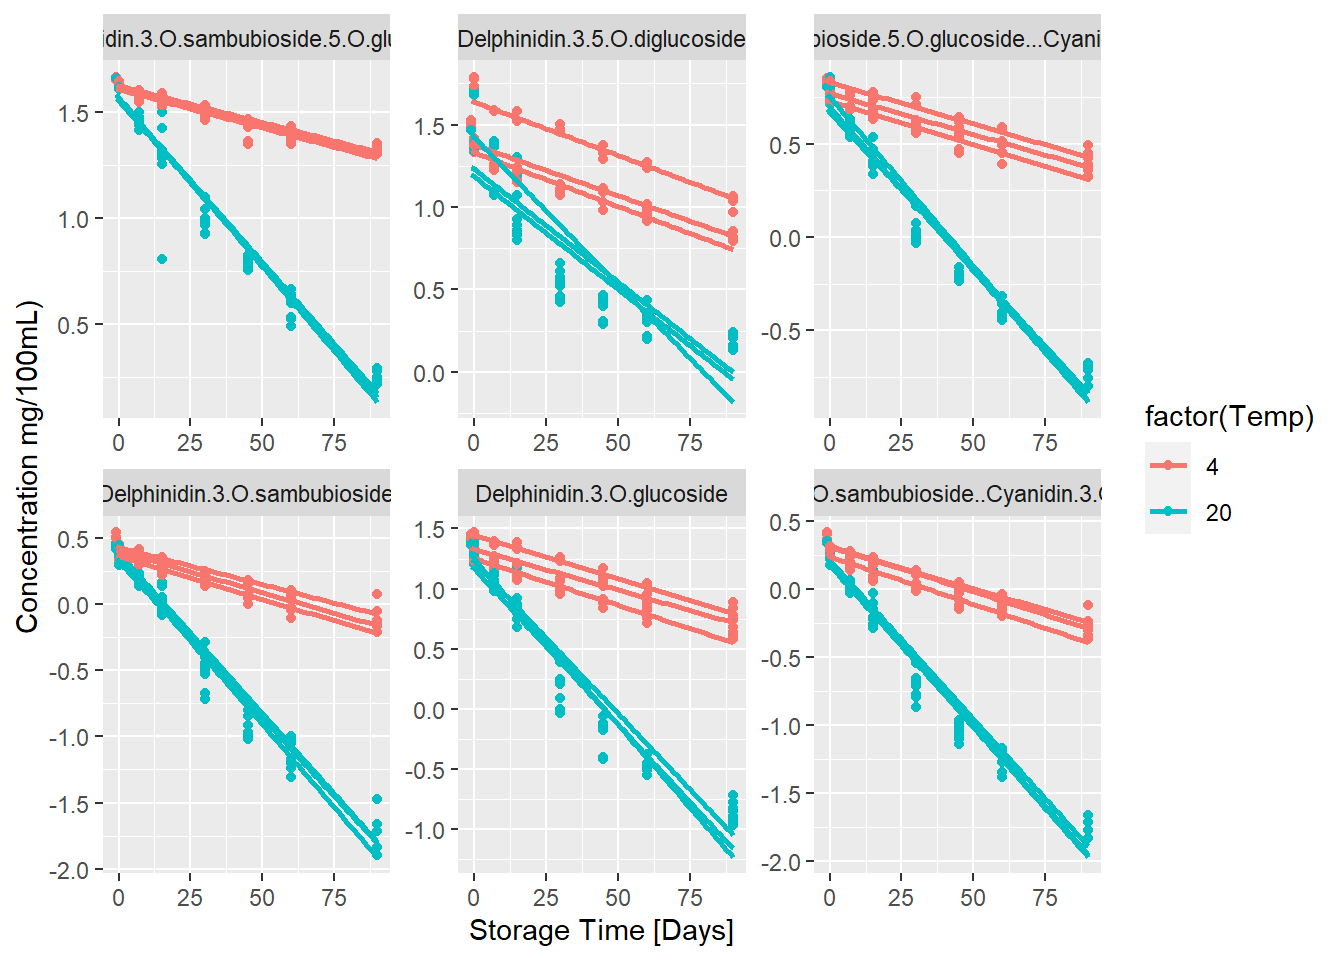
\includegraphics{firstModel_Jesus_files/figure-latex/first order-1.pdf}

De aquí podemos concluir que:

\begin{enumerate}
\def\labelenumi{\arabic{enumi}.}
\tightlist
\item
  La temperatura de almacenamiento es el factor más importante del
  estudio. Las diferencias entre colores son mucho mayores que las
  diferencias entre líneas del mismo color
\item
  Todas las antocianos salvo Delphinidin.3.5.O.diglucoside podrían
  razonablemente ser modeladas con un cinética de primer orden
  aparentemente.
\end{enumerate}

Procedemos a la primera modelización, una degradación de primer orden
aparente con una concentración residual y una energía de activación, un
modelo de referencia, con dependencia de la temperatura pero ni
procesado ni endulzante afectan, con la siguiente distribución, derivada
de la ecuación de Arrhenius y la cinética de primer orden:

\[C(t)_i \sim C_{\infty_i}+(C_{0_i}-C_{\infty_i})e^{(-e^{(lk_i-\frac{Ea_i}{R} \frac{1}{ T}-\frac{1}{T_{ref}})})t}\]
Donde \(C(t)_i\) es la concentracion del antocianino i a tiempo t y
\(C_{0_i}\) \(C_{\infty}\) \(lk_i\) and \(Ea_i\) son la concentracion
inicial, concentracion final, el logaritmo natural de la constante
aparente de primer orden y la energia de activacion para el antocianino
i. La temperatura de referencia es \(16^oC\) y la constante R es
\(0.008314 \frac{KJ}{Mol\cdot K}\).

\begin{Shaded}
\begin{Highlighting}[]
\NormalTok{ant.fm0}\OtherTok{\textless{}{-}}\FunctionTok{gnls}\NormalTok{(concentration}\SpecialCharTok{\textasciitilde{}}\NormalTok{Cinf}\SpecialCharTok{+}\NormalTok{(C0}\SpecialCharTok{{-}}\NormalTok{Cinf)}\SpecialCharTok{*}\FunctionTok{exp}\NormalTok{(}\SpecialCharTok{{-}}\FunctionTok{exp}\NormalTok{(lk}\SpecialCharTok{{-}}\NormalTok{Ea}\SpecialCharTok{/}\FloatTok{8.314e{-}3}\SpecialCharTok{*}\NormalTok{(}\DecValTok{1}\SpecialCharTok{/}\NormalTok{(Temp}\SpecialCharTok{+}\DecValTok{273}\NormalTok{)}\SpecialCharTok{{-}}\DecValTok{1}\SpecialCharTok{/}\NormalTok{(}\DecValTok{16}\SpecialCharTok{+}\DecValTok{273}\NormalTok{)))}\SpecialCharTok{*}\NormalTok{tiempo),}
              \AttributeTok{data=}\NormalTok{anthocyanins,}
              \AttributeTok{param=}\FunctionTok{list}\NormalTok{(C0}\SpecialCharTok{\textasciitilde{}}\NormalTok{compound,}
\NormalTok{                         Cinf}\SpecialCharTok{\textasciitilde{}}\NormalTok{compound,}
\NormalTok{                         lk}\SpecialCharTok{\textasciitilde{}}\NormalTok{compound,}
\NormalTok{                         Ea}\SpecialCharTok{\textasciitilde{}}\NormalTok{compound),}
              \AttributeTok{start=}\FunctionTok{c}\NormalTok{(}\AttributeTok{C0=}\FunctionTok{c}\NormalTok{(}\DecValTok{1}\NormalTok{,}\FunctionTok{rep}\NormalTok{(}\FloatTok{0.001}\NormalTok{,}\DecValTok{5}\NormalTok{)),}
                      \AttributeTok{Cinf=}\FunctionTok{c}\NormalTok{(}\DecValTok{0}\NormalTok{,}\FunctionTok{rep}\NormalTok{(}\FloatTok{0.001}\NormalTok{,}\DecValTok{5}\NormalTok{)),}
                      \AttributeTok{lk=}\FunctionTok{c}\NormalTok{(}\FloatTok{0.01}\NormalTok{,}\FunctionTok{rep}\NormalTok{(}\FloatTok{0.001}\NormalTok{,}\DecValTok{5}\NormalTok{)),}
                      \AttributeTok{Ea=}\FunctionTok{c}\NormalTok{(}\DecValTok{10}\NormalTok{,}\FunctionTok{rep}\NormalTok{(}\FloatTok{0.001}\NormalTok{,}\DecValTok{5}\NormalTok{)))}
\NormalTok{)}
\FunctionTok{summary}\NormalTok{(ant.fm0,}\AttributeTok{cor=}\NormalTok{F)}
\end{Highlighting}
\end{Shaded}

\emph{Modelizacion de la co-varianza}

Con el diseño experimental se pueden estimar los efectos principales de
las variables endulzante y procesado para compuesto. La estimacion de
interacciones y los terminos de orden superior requeriria completar este
diseño.

En este modelo endulzante y procesado son efectos iguales para todos los
compuestos.

\begin{Shaded}
\begin{Highlighting}[]
\NormalTok{ant.fm1}\OtherTok{\textless{}{-}}\FunctionTok{gnls}\NormalTok{(concentration}\SpecialCharTok{\textasciitilde{}}\NormalTok{Cinf}\SpecialCharTok{+}\NormalTok{(C0}\SpecialCharTok{{-}}\NormalTok{Cinf)}\SpecialCharTok{*}\FunctionTok{exp}\NormalTok{(}\SpecialCharTok{{-}}\FunctionTok{exp}\NormalTok{(lk}\SpecialCharTok{{-}}\NormalTok{Ea}\SpecialCharTok{/}\FloatTok{8.314e{-}3}\SpecialCharTok{*}\NormalTok{(}\DecValTok{1}\SpecialCharTok{/}\NormalTok{(Temp}\SpecialCharTok{+}\DecValTok{273}\NormalTok{)}\SpecialCharTok{{-}}\DecValTok{1}\SpecialCharTok{/}\NormalTok{(}\DecValTok{16}\SpecialCharTok{+}\DecValTok{273}\NormalTok{)))}\SpecialCharTok{*}\NormalTok{tiempo),}
              \AttributeTok{data=}\NormalTok{anthocyanins,}
              \AttributeTok{param=}\FunctionTok{list}\NormalTok{(C0}\SpecialCharTok{\textasciitilde{}}\NormalTok{compound}\SpecialCharTok{+}\NormalTok{sweetener}\SpecialCharTok{+}\NormalTok{processing,}
\NormalTok{                         Cinf}\SpecialCharTok{\textasciitilde{}}\NormalTok{compound}\SpecialCharTok{+}\NormalTok{sweetener}\SpecialCharTok{+}\NormalTok{processing,}
\NormalTok{                         lk}\SpecialCharTok{\textasciitilde{}}\NormalTok{compound}\SpecialCharTok{+}\NormalTok{sweetener}\SpecialCharTok{+}\NormalTok{processing,}
\NormalTok{                         Ea}\SpecialCharTok{\textasciitilde{}}\DecValTok{1}\NormalTok{),}
              \AttributeTok{start=}\FunctionTok{c}\NormalTok{(}\AttributeTok{C0=}\FunctionTok{c}\NormalTok{(}\FunctionTok{coef}\NormalTok{(ant.fm0)[}\DecValTok{1}\SpecialCharTok{:}\DecValTok{6}\NormalTok{],}\FunctionTok{rep}\NormalTok{(}\FloatTok{0.001}\NormalTok{,}\DecValTok{3}\NormalTok{)),}
                      \AttributeTok{Cinf=}\FunctionTok{c}\NormalTok{(}\FunctionTok{coef}\NormalTok{(ant.fm0)[}\DecValTok{7}\SpecialCharTok{:}\DecValTok{12}\NormalTok{],}\FunctionTok{rep}\NormalTok{(}\FloatTok{0.001}\NormalTok{,}\DecValTok{3}\NormalTok{)),}
                      \AttributeTok{lk=}\FunctionTok{c}\NormalTok{(}\FunctionTok{coef}\NormalTok{(ant.fm0)[}\DecValTok{13}\SpecialCharTok{:}\DecValTok{18}\NormalTok{],}\FunctionTok{rep}\NormalTok{(}\FloatTok{0.001}\NormalTok{,}\DecValTok{3}\NormalTok{)),}
                      \AttributeTok{Ea=}\FunctionTok{c}\NormalTok{(}\FunctionTok{coef}\NormalTok{(ant.fm0)[}\DecValTok{19}\NormalTok{])}
\NormalTok{                      )}
\NormalTok{)}
\FunctionTok{summary}\NormalTok{(ant.fm1)}
\end{Highlighting}
\end{Shaded}

Ahora intentaremos estimar los diferentes coeficientes de constantes
entre diferentes componentes y condiciones de procesamiento

\begin{Shaded}
\begin{Highlighting}[]
\NormalTok{ant.fm2}\OtherTok{\textless{}{-}}\FunctionTok{gnls}\NormalTok{(concentration}\SpecialCharTok{\textasciitilde{}}\NormalTok{Cinf}\SpecialCharTok{+}\NormalTok{(C0}\SpecialCharTok{{-}}\NormalTok{Cinf)}\SpecialCharTok{*}\FunctionTok{exp}\NormalTok{(}\SpecialCharTok{{-}}\FunctionTok{exp}\NormalTok{(lk}\SpecialCharTok{{-}}\NormalTok{Ea}\SpecialCharTok{/}\FloatTok{8.314e{-}3}\SpecialCharTok{*}\NormalTok{(}\DecValTok{1}\SpecialCharTok{/}\NormalTok{(Temp}\SpecialCharTok{+}\DecValTok{273}\NormalTok{)}\SpecialCharTok{{-}}\DecValTok{1}\SpecialCharTok{/}\NormalTok{(}\DecValTok{16}\SpecialCharTok{+}\DecValTok{273}\NormalTok{)))}\SpecialCharTok{*}\NormalTok{tiempo),}
               \AttributeTok{data=}\NormalTok{anthocyanins,}
               \AttributeTok{param=}\FunctionTok{list}\NormalTok{(C0}\SpecialCharTok{\textasciitilde{}}\NormalTok{compound}\SpecialCharTok{+}\NormalTok{sweetener}\SpecialCharTok{+}\NormalTok{processing,}
\NormalTok{                          Cinf}\SpecialCharTok{\textasciitilde{}}\NormalTok{compound}\SpecialCharTok{+}\NormalTok{sweetener}\SpecialCharTok{+}\NormalTok{processing,}
\NormalTok{                          lk}\SpecialCharTok{\textasciitilde{}}\NormalTok{compound}\SpecialCharTok{+}\NormalTok{sweetener}\SpecialCharTok{+}\NormalTok{compound}\SpecialCharTok{:}\NormalTok{processing,}
\NormalTok{                          Ea}\SpecialCharTok{\textasciitilde{}}\NormalTok{compound),}
               \AttributeTok{start=}\FunctionTok{c}\NormalTok{(}\AttributeTok{C0=}\FunctionTok{c}\NormalTok{(}\FunctionTok{coef}\NormalTok{(ant.fm0)[}\DecValTok{1}\SpecialCharTok{:}\DecValTok{6}\NormalTok{],}\FunctionTok{rep}\NormalTok{(}\FloatTok{0.001}\NormalTok{,}\DecValTok{3}\NormalTok{)),}
                       \AttributeTok{Cinf=}\FunctionTok{c}\NormalTok{(}\FunctionTok{coef}\NormalTok{(ant.fm0)[}\DecValTok{7}\SpecialCharTok{:}\DecValTok{12}\NormalTok{],}\FunctionTok{rep}\NormalTok{(}\FloatTok{0.001}\NormalTok{,}\DecValTok{3}\NormalTok{)),}
                       \AttributeTok{lk=}\FunctionTok{c}\NormalTok{(}\FunctionTok{coef}\NormalTok{(ant.fm0)[}\DecValTok{13}\SpecialCharTok{:}\DecValTok{18}\NormalTok{],}\FunctionTok{rep}\NormalTok{(}\FloatTok{0.001}\NormalTok{,}\DecValTok{13}\NormalTok{)),}
                       \AttributeTok{Ea=}\FunctionTok{c}\NormalTok{(}\FunctionTok{coef}\NormalTok{(ant.fm0)[}\DecValTok{19}\NormalTok{],}\FunctionTok{rep}\NormalTok{(}\FloatTok{0.001}\NormalTok{,}\DecValTok{5}\NormalTok{))}
\NormalTok{               )}
\NormalTok{)}
\FunctionTok{summary}\NormalTok{(ant.fm2)}
\end{Highlighting}
\end{Shaded}

Obtenemos aproximadamente cuatro parámetros significativos. Ea es solo
diferente en D.3.5.0.diglucosido

Realizamos un análisis anova para los resultados de los modelos:

\begin{Shaded}
\begin{Highlighting}[]
\FunctionTok{anova}\NormalTok{(ant.fm0,ant.fm1,ant.fm2)}
\end{Highlighting}
\end{Shaded}

\begin{verbatim}
##         Model df        AIC       BIC    logLik   Test  L.Ratio p-value
## ant.fm0     1 25   71.25632 190.29564 -10.62816                        
## ant.fm1     2 29 -177.22100 -39.13539 117.61050 1 vs 2 256.4773  <.0001
## ant.fm2     3 44 -291.24731 -81.73811 189.62366 2 vs 3 144.0263  <.0001
\end{verbatim}

Las mejoras en los modelos son muy significativas y mejoran el ruido

Realizamos un cuarto modelo, con los coeficientes de los factores en
todas las variables

\begin{Shaded}
\begin{Highlighting}[]
\NormalTok{ant.fm3}\OtherTok{\textless{}{-}}\FunctionTok{gnls}\NormalTok{(concentration}\SpecialCharTok{\textasciitilde{}}\NormalTok{Cinf}\SpecialCharTok{+}\NormalTok{(C0}\SpecialCharTok{{-}}\NormalTok{Cinf)}\SpecialCharTok{*}\FunctionTok{exp}\NormalTok{(}\SpecialCharTok{{-}}\FunctionTok{exp}\NormalTok{(lk}\SpecialCharTok{{-}}\NormalTok{Ea}\SpecialCharTok{/}\FloatTok{8.314e{-}3}\SpecialCharTok{*}\NormalTok{(}\DecValTok{1}\SpecialCharTok{/}\NormalTok{(Temp}\SpecialCharTok{+}\DecValTok{273}\NormalTok{)}\SpecialCharTok{{-}}\DecValTok{1}\SpecialCharTok{/}\NormalTok{(}\DecValTok{16}\SpecialCharTok{+}\DecValTok{273}\NormalTok{)))}\SpecialCharTok{*}\NormalTok{tiempo),}
               \AttributeTok{data=}\NormalTok{anthocyanins,}
               \AttributeTok{param=}\FunctionTok{list}\NormalTok{(C0}\SpecialCharTok{\textasciitilde{}}\NormalTok{compound}\SpecialCharTok{+}\NormalTok{compound}\SpecialCharTok{:}\NormalTok{sweetener}\SpecialCharTok{+}\NormalTok{compound}\SpecialCharTok{:}\NormalTok{processing,}
\NormalTok{                          Cinf}\SpecialCharTok{\textasciitilde{}}\NormalTok{compound}\SpecialCharTok{+}\NormalTok{compound}\SpecialCharTok{:}\NormalTok{sweetener}\SpecialCharTok{+}\NormalTok{compound}\SpecialCharTok{:}\NormalTok{processing,}
\NormalTok{                          lk}\SpecialCharTok{\textasciitilde{}}\NormalTok{compound}\SpecialCharTok{+}\NormalTok{compound}\SpecialCharTok{:}\NormalTok{sweetener}\SpecialCharTok{+}\NormalTok{compound}\SpecialCharTok{:}\NormalTok{processing,}
\NormalTok{                          Ea}\SpecialCharTok{\textasciitilde{}}\NormalTok{compound),}
               \AttributeTok{start=}\FunctionTok{c}\NormalTok{(}\AttributeTok{C0=}\FunctionTok{c}\NormalTok{(}\FunctionTok{coef}\NormalTok{(ant.fm0)[}\DecValTok{1}\SpecialCharTok{:}\DecValTok{6}\NormalTok{],}\FunctionTok{rep}\NormalTok{(}\FloatTok{0.001}\NormalTok{,}\DecValTok{18}\NormalTok{)),}
                       \AttributeTok{Cinf=}\FunctionTok{c}\NormalTok{(}\FunctionTok{coef}\NormalTok{(ant.fm0)[}\DecValTok{7}\SpecialCharTok{:}\DecValTok{12}\NormalTok{],}\FunctionTok{rep}\NormalTok{(}\FloatTok{0.001}\NormalTok{,}\DecValTok{18}\NormalTok{)),}
                       \AttributeTok{lk=}\FunctionTok{c}\NormalTok{(}\FunctionTok{coef}\NormalTok{(ant.fm0)[}\DecValTok{13}\SpecialCharTok{:}\DecValTok{18}\NormalTok{],}\FunctionTok{rep}\NormalTok{(}\FloatTok{0.001}\NormalTok{,}\DecValTok{18}\NormalTok{)),}
                       \AttributeTok{Ea=}\FunctionTok{c}\NormalTok{(}\FunctionTok{coef}\NormalTok{(ant.fm0)[}\DecValTok{13}\SpecialCharTok{:}\DecValTok{18}\NormalTok{])}
\NormalTok{               )}
\NormalTok{)}
\FunctionTok{screenreg}\NormalTok{(ant.fm3,}\AttributeTok{single.row=}\NormalTok{T,}\AttributeTok{ci.force=}\NormalTok{T)}
\end{Highlighting}
\end{Shaded}

De nuevo, evaluamos los modelos con anova, y miramos el r2 del cuarto
modelo

\begin{Shaded}
\begin{Highlighting}[]
\FunctionTok{anova}\NormalTok{(ant.fm0,ant.fm1,ant.fm2,ant.fm3)}
\end{Highlighting}
\end{Shaded}

\begin{verbatim}
##         Model df       AIC        BIC   logLik   Test  L.Ratio p-value
## ant.fm0     1 25   71.2563  190.29564 -10.6282                        
## ant.fm1     2 29 -177.2210  -39.13539 117.6105 1 vs 2 256.4773  <.0001
## ant.fm2     3 44 -291.2473  -81.73811 189.6237 2 vs 3 144.0263  <.0001
## ant.fm3     4 79 -625.5766 -249.41238 391.7883 3 vs 4 404.3293  <.0001
\end{verbatim}

\begin{Shaded}
\begin{Highlighting}[]
\FunctionTok{r2}\NormalTok{(ant.fm3)}
\end{Highlighting}
\end{Shaded}

\begin{verbatim}
## [1] 0.9886055 0.9874892
\end{verbatim}

Realizamos gráficas de diagnóstico para el cuarto modelo

\begin{Shaded}
\begin{Highlighting}[]
\FunctionTok{plot}\NormalTok{(ant.fm3)}
\end{Highlighting}
\end{Shaded}

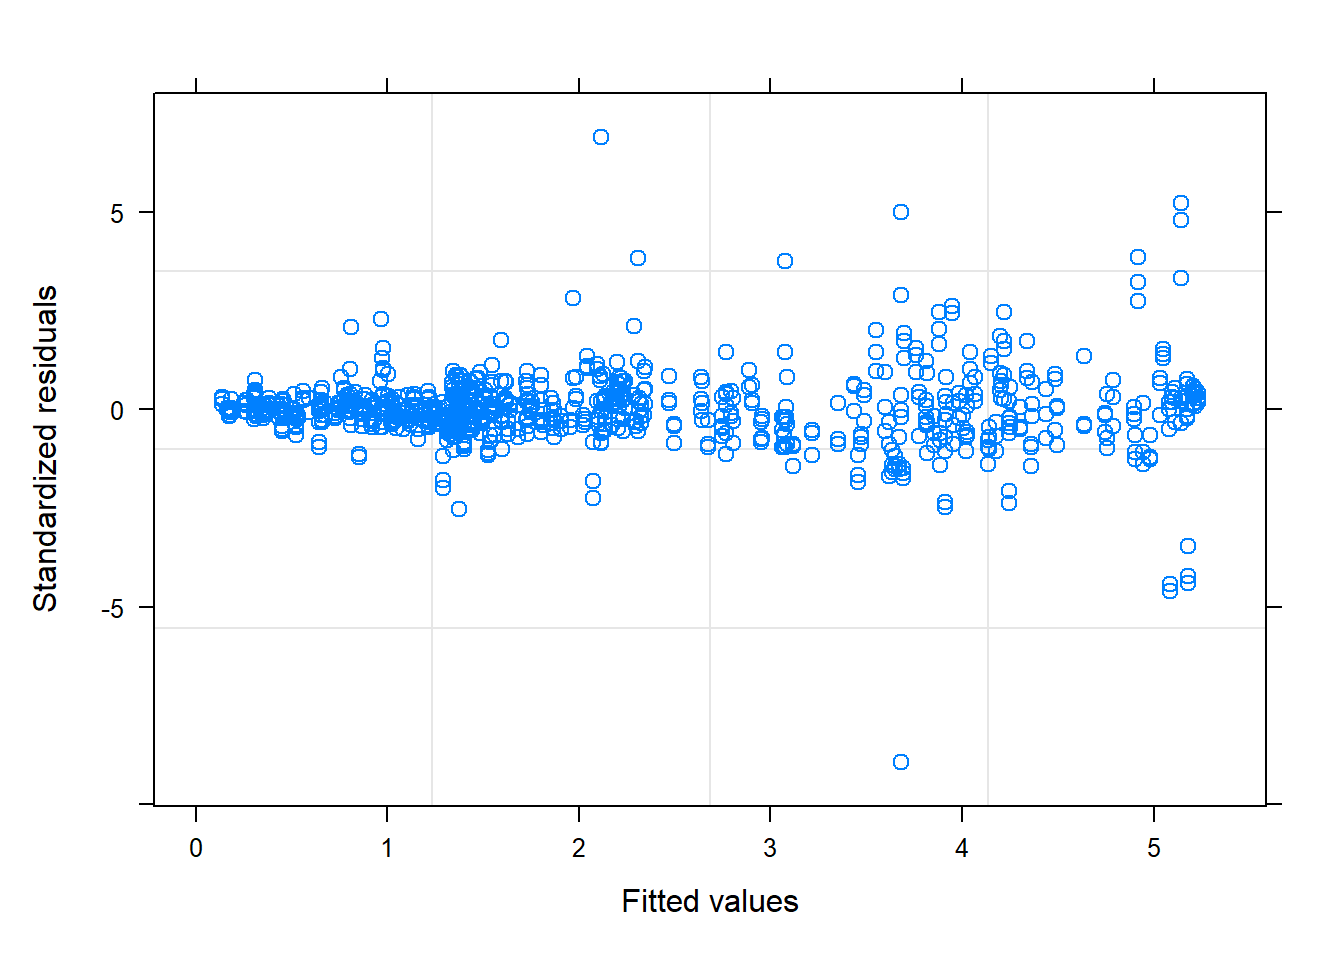
\includegraphics{firstModel_Jesus_files/figure-latex/diagnostic tables-1.pdf}

\begin{Shaded}
\begin{Highlighting}[]
\FunctionTok{qqnorm}\NormalTok{(ant.fm3)}
\end{Highlighting}
\end{Shaded}

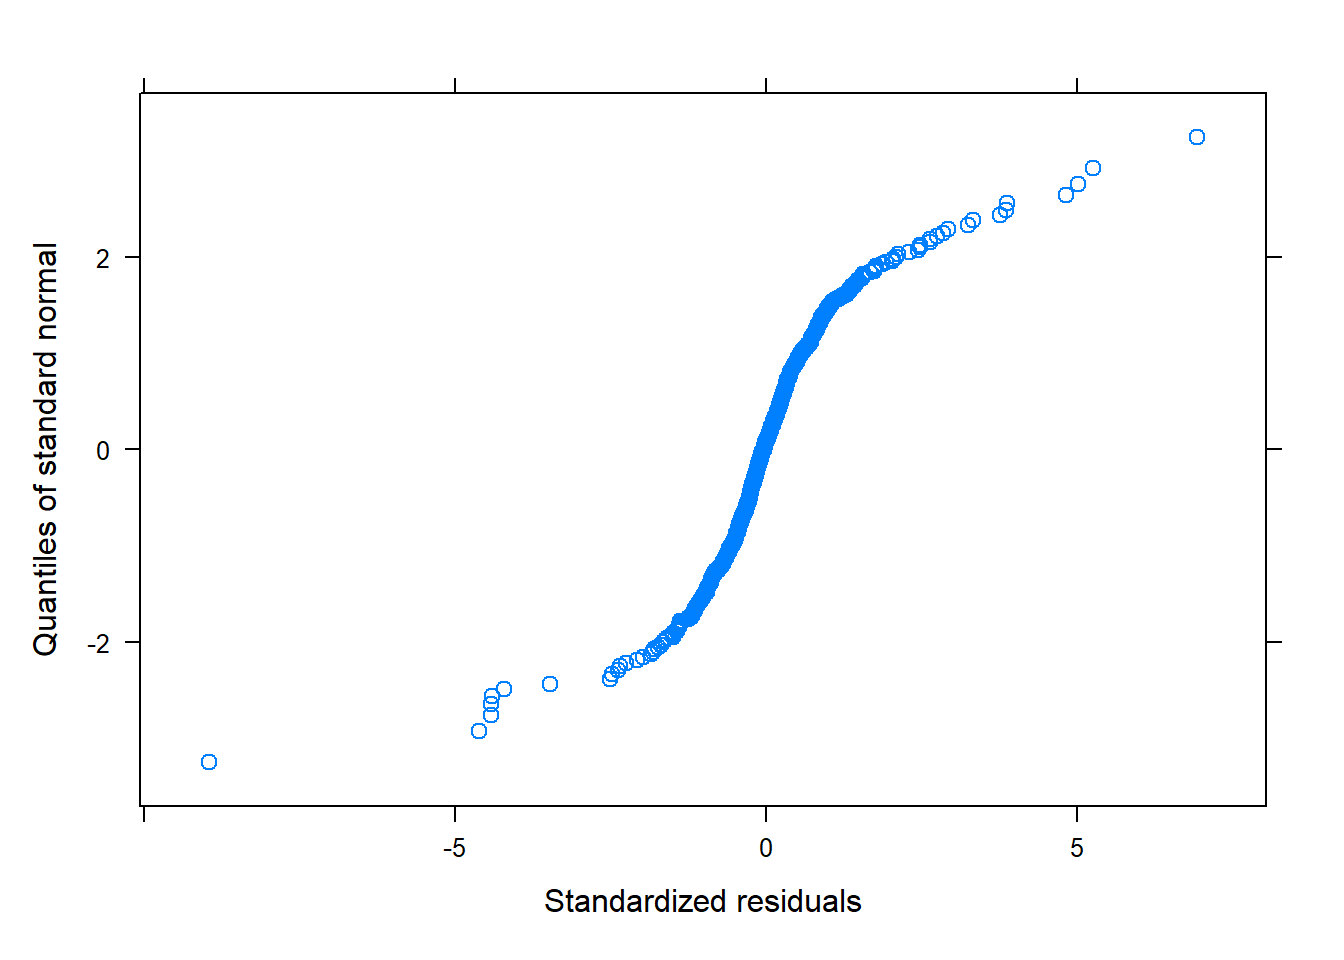
\includegraphics{firstModel_Jesus_files/figure-latex/diagnostic tables-2.pdf}

\begin{Shaded}
\begin{Highlighting}[]
\FunctionTok{plot}\NormalTok{(ant.fm3,}\FunctionTok{resid}\NormalTok{(.)}\SpecialCharTok{\textasciitilde{}}\NormalTok{Temp)}
\end{Highlighting}
\end{Shaded}

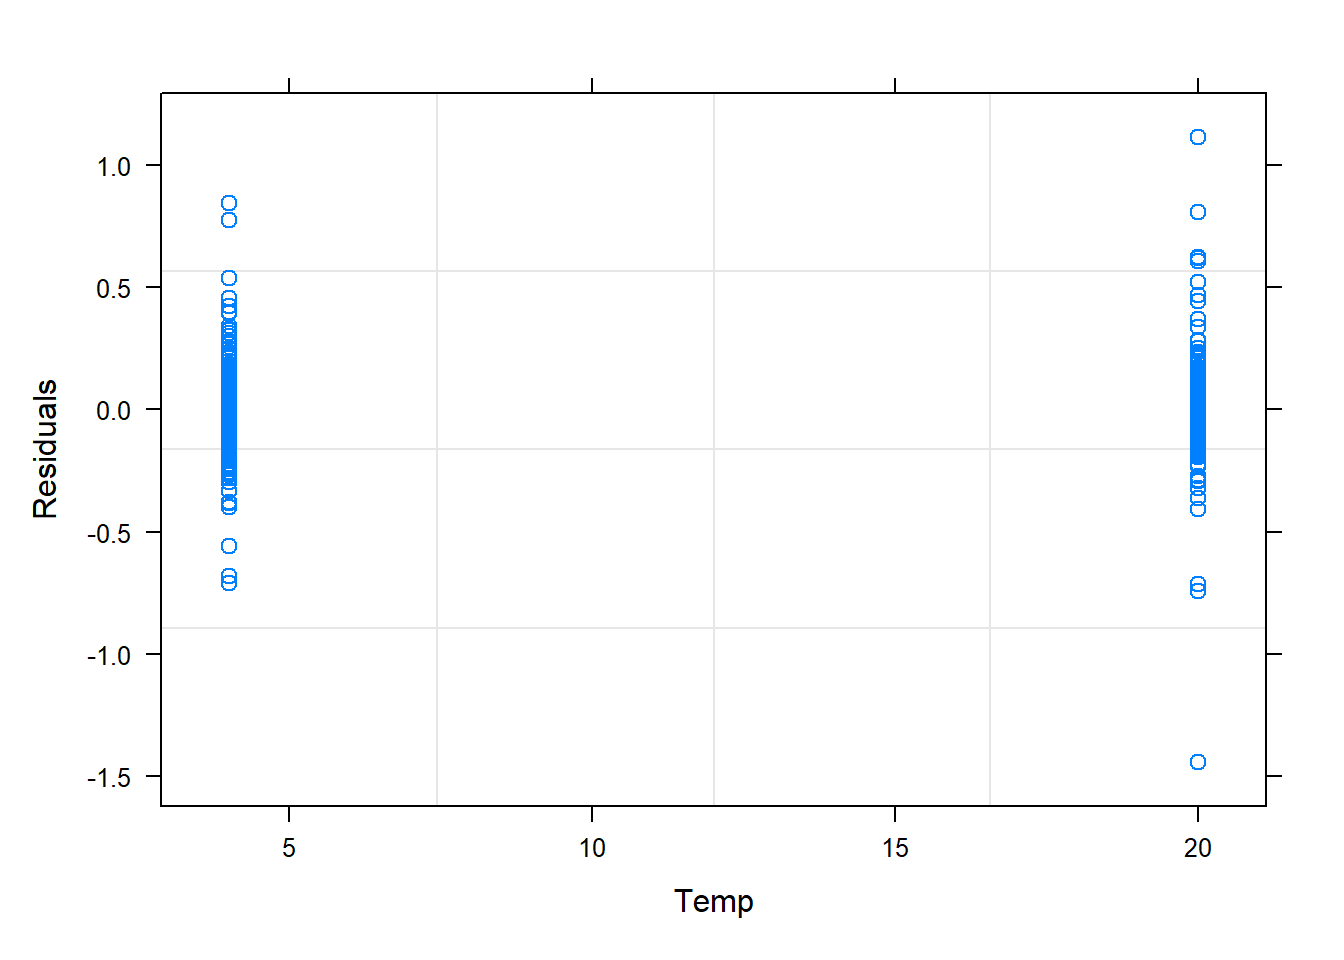
\includegraphics{firstModel_Jesus_files/figure-latex/diagnostic tables-3.pdf}

\begin{Shaded}
\begin{Highlighting}[]
\FunctionTok{plot}\NormalTok{(ant.fm3,compound}\SpecialCharTok{\textasciitilde{}}\FunctionTok{resid}\NormalTok{(.))}
\end{Highlighting}
\end{Shaded}

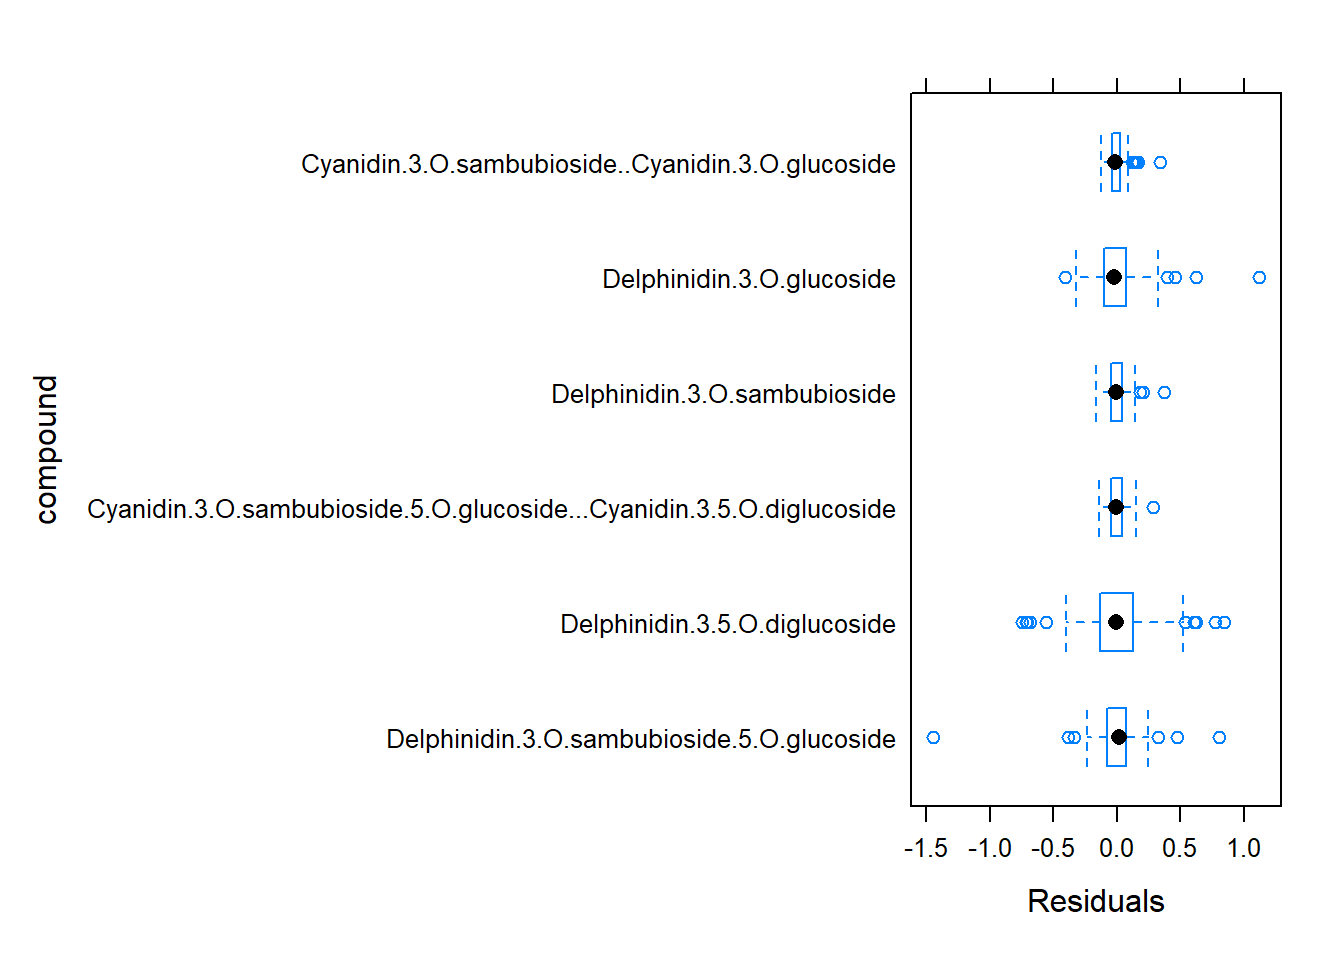
\includegraphics{firstModel_Jesus_files/figure-latex/diagnostic tables-4.pdf}

\begin{Shaded}
\begin{Highlighting}[]
\FunctionTok{plot}\NormalTok{(ant.fm3,processing}\SpecialCharTok{\textasciitilde{}}\FunctionTok{resid}\NormalTok{(.))}
\end{Highlighting}
\end{Shaded}

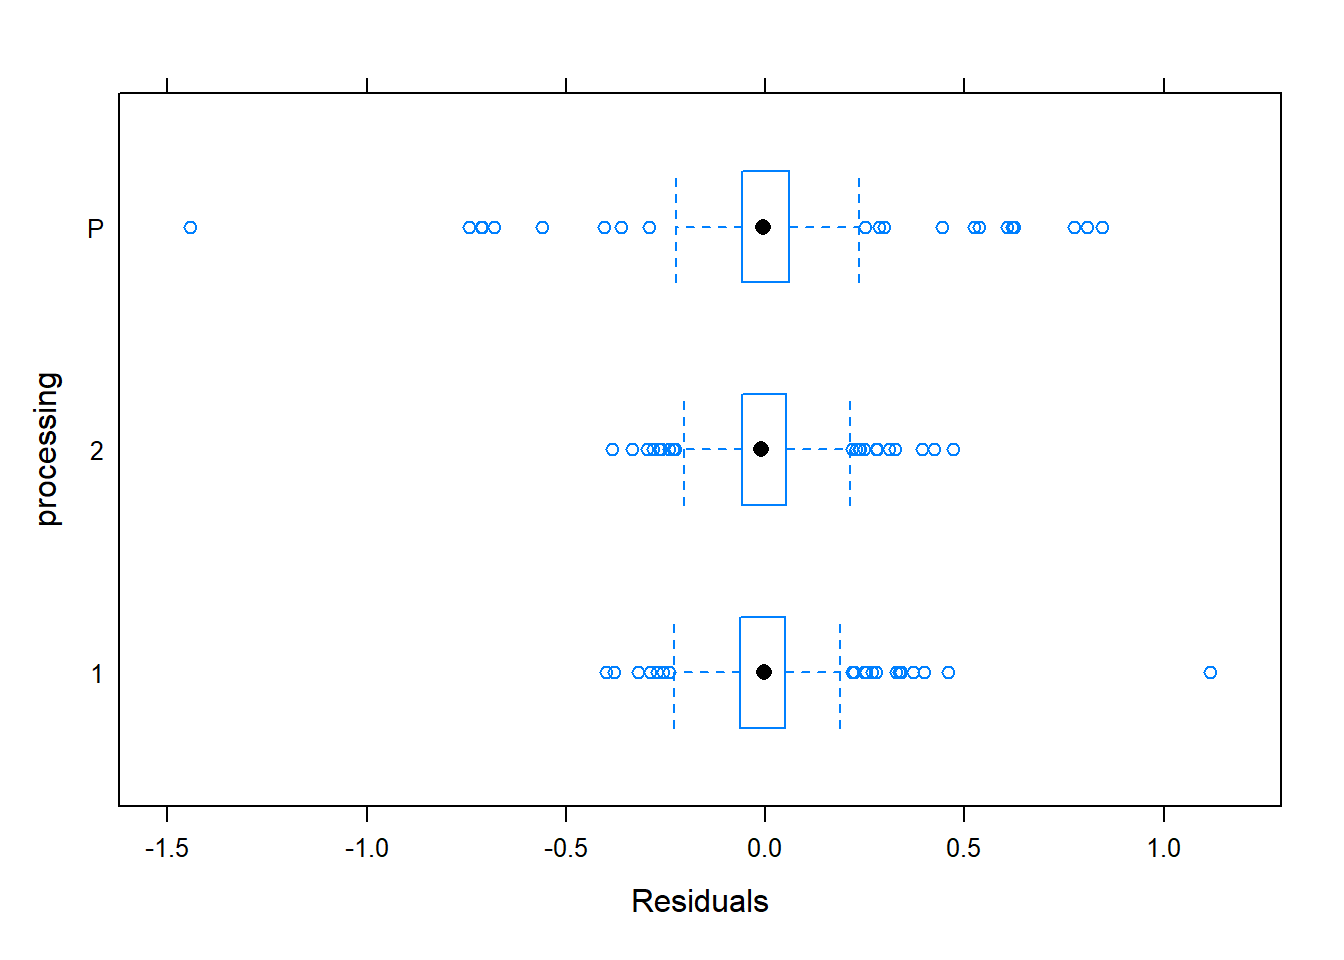
\includegraphics{firstModel_Jesus_files/figure-latex/diagnostic tables-5.pdf}

\begin{Shaded}
\begin{Highlighting}[]
\FunctionTok{plot}\NormalTok{(ant.fm3,sweetener}\SpecialCharTok{\textasciitilde{}}\FunctionTok{resid}\NormalTok{(.))}
\end{Highlighting}
\end{Shaded}

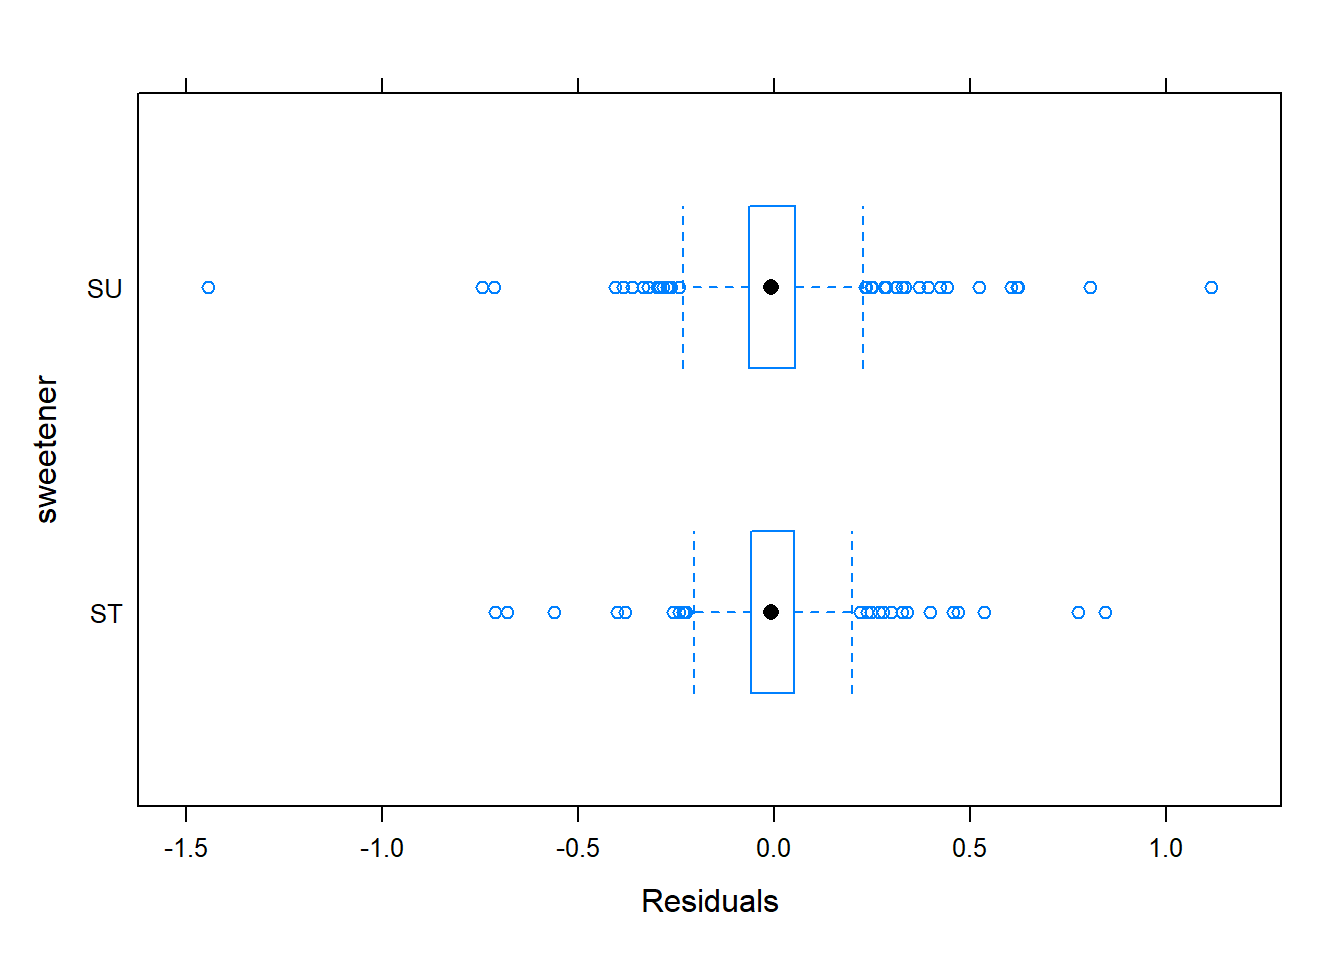
\includegraphics{firstModel_Jesus_files/figure-latex/diagnostic tables-6.pdf}

Gráfica 1, Residuos vs Ajustes: Se confirma que los residuos se
distribuyen aleatoriamente y con varianza constante.

Gráfica 2, probabilidad normal de residuos: Se confirma que los residuos
siguen una probabilidad normal

Gráficas 3,4,5 y 6, residuos vs variables: Las variables tienen
importancia en el modelo al observar patrones no aleatorios

Creamos una tabla a partir de los resultados, la guardamos como
``anthocyanins.html'' y generamos gráficas para evaluar las predicciones
del cuarto modelo, viéndose la predicción del ajuste en las lineas y los
datos del experimento en puntos:

\begin{Shaded}
\begin{Highlighting}[]
\NormalTok{list.of.compound.fit}\OtherTok{\textless{}{-}}\FunctionTok{list}\NormalTok{()}
\NormalTok{list.of.r2adj}\OtherTok{\textless{}{-}}\FunctionTok{list}\NormalTok{()}
\ControlFlowTok{for}\NormalTok{ (i }\ControlFlowTok{in} \FunctionTok{levels}\NormalTok{(}\FunctionTok{factor}\NormalTok{(anthocyanins}\SpecialCharTok{$}\NormalTok{compound)))\{}
  \CommentTok{\#print(i)}
\NormalTok{  list.of.compound.fit[[i]]}\OtherTok{\textless{}{-}}\FunctionTok{gnls}\NormalTok{(concentration}\SpecialCharTok{\textasciitilde{}}\NormalTok{Cinf}\SpecialCharTok{+}\NormalTok{(C0}\SpecialCharTok{{-}}\NormalTok{Cinf)}\SpecialCharTok{*}\FunctionTok{exp}\NormalTok{(}\SpecialCharTok{{-}}\FunctionTok{exp}\NormalTok{(lk}\SpecialCharTok{{-}}\NormalTok{Ea}\SpecialCharTok{/}\FloatTok{8.314e{-}3}\SpecialCharTok{*}\NormalTok{(}\DecValTok{1}\SpecialCharTok{/}\NormalTok{(Temp}\SpecialCharTok{+}\DecValTok{273}\NormalTok{)}\SpecialCharTok{{-}}\DecValTok{1}\SpecialCharTok{/}\NormalTok{(}\DecValTok{16}\SpecialCharTok{+}\DecValTok{273}\NormalTok{)))}\SpecialCharTok{*}\NormalTok{tiempo),}
                                  \AttributeTok{data=}\FunctionTok{subset}\NormalTok{(anthocyanins,compound}\SpecialCharTok{==}\NormalTok{i),}
                                  \AttributeTok{param=}\FunctionTok{list}\NormalTok{(C0}\SpecialCharTok{\textasciitilde{}}\NormalTok{sweetener}\SpecialCharTok{+}\NormalTok{processing,}
\NormalTok{                                             Cinf}\SpecialCharTok{\textasciitilde{}}\NormalTok{sweetener}\SpecialCharTok{+}\NormalTok{processing,}
\NormalTok{                                             lk}\SpecialCharTok{\textasciitilde{}}\NormalTok{sweetener}\SpecialCharTok{+}\NormalTok{processing,}
\NormalTok{                                             Ea}\SpecialCharTok{\textasciitilde{}}\DecValTok{1}\NormalTok{),}
                                  \AttributeTok{start=}\FunctionTok{c}\NormalTok{(}\AttributeTok{C0=}\FunctionTok{c}\NormalTok{(}\FloatTok{5.05}\NormalTok{,}\FunctionTok{rep}\NormalTok{(}\FloatTok{0.001}\NormalTok{,}\DecValTok{3}\NormalTok{)),}
                                          \AttributeTok{Cinf=}\FunctionTok{c}\NormalTok{(}\DecValTok{0}\NormalTok{,}\FunctionTok{rep}\NormalTok{(}\FloatTok{0.001}\NormalTok{,}\DecValTok{3}\NormalTok{)),}
                                          \AttributeTok{lk=}\FunctionTok{c}\NormalTok{(}\SpecialCharTok{{-}}\FloatTok{4.38}\NormalTok{,}\FunctionTok{rep}\NormalTok{(}\FloatTok{0.001}\NormalTok{,}\DecValTok{3}\NormalTok{)),}
                                          \AttributeTok{Ea=}\FunctionTok{c}\NormalTok{(}\DecValTok{67}\NormalTok{)}
\NormalTok{                                  )}
\NormalTok{  )}
\NormalTok{  list.of.r2adj[[i]]}\OtherTok{\textless{}{-}}\FunctionTok{round}\NormalTok{(}\FunctionTok{r2}\NormalTok{(list.of.compound.fit[[i]])[}\DecValTok{2}\NormalTok{],}\DecValTok{3}\NormalTok{)}
\NormalTok{\}}

\CommentTok{\#screenreg(list.of.compound.fit,single.row=T,ci.force=T)}
\end{Highlighting}
\end{Shaded}

\newpage
\begin{landscape}

\begin{verbatim}
## The table was written to the file 'anthocyanins.html'.
\end{verbatim}

\end{landscape}

\begin{Shaded}
\begin{Highlighting}[]
\NormalTok{anthocyanins}\SpecialCharTok{$}\NormalTok{grouping}\OtherTok{\textless{}{-}}\FunctionTok{with}\NormalTok{(anthocyanins,sweetener}\SpecialCharTok{:}\NormalTok{processing}\SpecialCharTok{:}\FunctionTok{factor}\NormalTok{(Temp))}
\NormalTok{ant.pred}\OtherTok{\textless{}{-}}\FunctionTok{expand.grid}\NormalTok{(}\AttributeTok{tiempo=}\FunctionTok{seq}\NormalTok{(}\DecValTok{0}\NormalTok{,}\DecValTok{90}\NormalTok{,}\AttributeTok{length=}\DecValTok{50}\NormalTok{),}
                       \AttributeTok{compound=}\FunctionTok{levels}\NormalTok{(}\FunctionTok{factor}\NormalTok{(anthocyanins}\SpecialCharTok{$}\NormalTok{compound)),}
                       \AttributeTok{grouping=}\FunctionTok{levels}\NormalTok{(}\FunctionTok{factor}\NormalTok{(anthocyanins}\SpecialCharTok{$}\NormalTok{grouping))}
\NormalTok{                       )}
\NormalTok{ant.pred}\SpecialCharTok{$}\NormalTok{sweetener}\OtherTok{\textless{}{-}}\FunctionTok{factor}\NormalTok{(}\FunctionTok{with}\NormalTok{(ant.pred,}\FunctionTok{substr}\NormalTok{(grouping,}\DecValTok{0}\NormalTok{,}\DecValTok{2}\NormalTok{)))}
\NormalTok{ant.pred}\SpecialCharTok{$}\NormalTok{processing}\OtherTok{\textless{}{-}}\FunctionTok{factor}\NormalTok{(}\FunctionTok{with}\NormalTok{(ant.pred,}\FunctionTok{substr}\NormalTok{(grouping,}\DecValTok{4}\NormalTok{,}\DecValTok{4}\NormalTok{)))}
\NormalTok{ant.pred}\SpecialCharTok{$}\NormalTok{Temp}\OtherTok{\textless{}{-}}\FunctionTok{as.numeric}\NormalTok{(}\FunctionTok{with}\NormalTok{(ant.pred,}\FunctionTok{substr}\NormalTok{(grouping,}\DecValTok{6}\NormalTok{,}\DecValTok{8}\NormalTok{)))}
\NormalTok{ant.pred}\SpecialCharTok{$}\NormalTok{concentration}\OtherTok{\textless{}{-}}\FunctionTok{predict}\NormalTok{(ant.fm3,}\AttributeTok{newdata =}\NormalTok{ ant.pred)}
\FunctionTok{ggplot}\NormalTok{(anthocyanins, }
       \FunctionTok{aes}\NormalTok{(}\AttributeTok{x =}\NormalTok{ tiempo, }\AttributeTok{y =}\NormalTok{ concentration, }\AttributeTok{col =}\NormalTok{grouping)) }\SpecialCharTok{+}
  \FunctionTok{facet\_wrap}\NormalTok{(compound}\SpecialCharTok{\textasciitilde{}}\NormalTok{.,}\AttributeTok{scales=}\StringTok{"free"}\NormalTok{)}\SpecialCharTok{+}
  \FunctionTok{geom\_point}\NormalTok{()}\SpecialCharTok{+}\FunctionTok{geom\_line}\NormalTok{(}\AttributeTok{data=}\NormalTok{ant.pred,}\FunctionTok{aes}\NormalTok{(}\AttributeTok{x=}\NormalTok{tiempo,}\AttributeTok{y=}\NormalTok{concentration,}\AttributeTok{col=}\NormalTok{grouping))}\SpecialCharTok{+}
  \FunctionTok{ggtitle}\NormalTok{(}\StringTok{"Degradation kinetic modelled from experimental (lines) vs experimental (dots)"}\NormalTok{)}\SpecialCharTok{+}
  \FunctionTok{xlab}\NormalTok{(}\StringTok{"Storage Time [Days]"}\NormalTok{)}\SpecialCharTok{+}\FunctionTok{ylab}\NormalTok{(}\StringTok{"Concentration [mg/100mL]"}\NormalTok{)}
\end{Highlighting}
\end{Shaded}

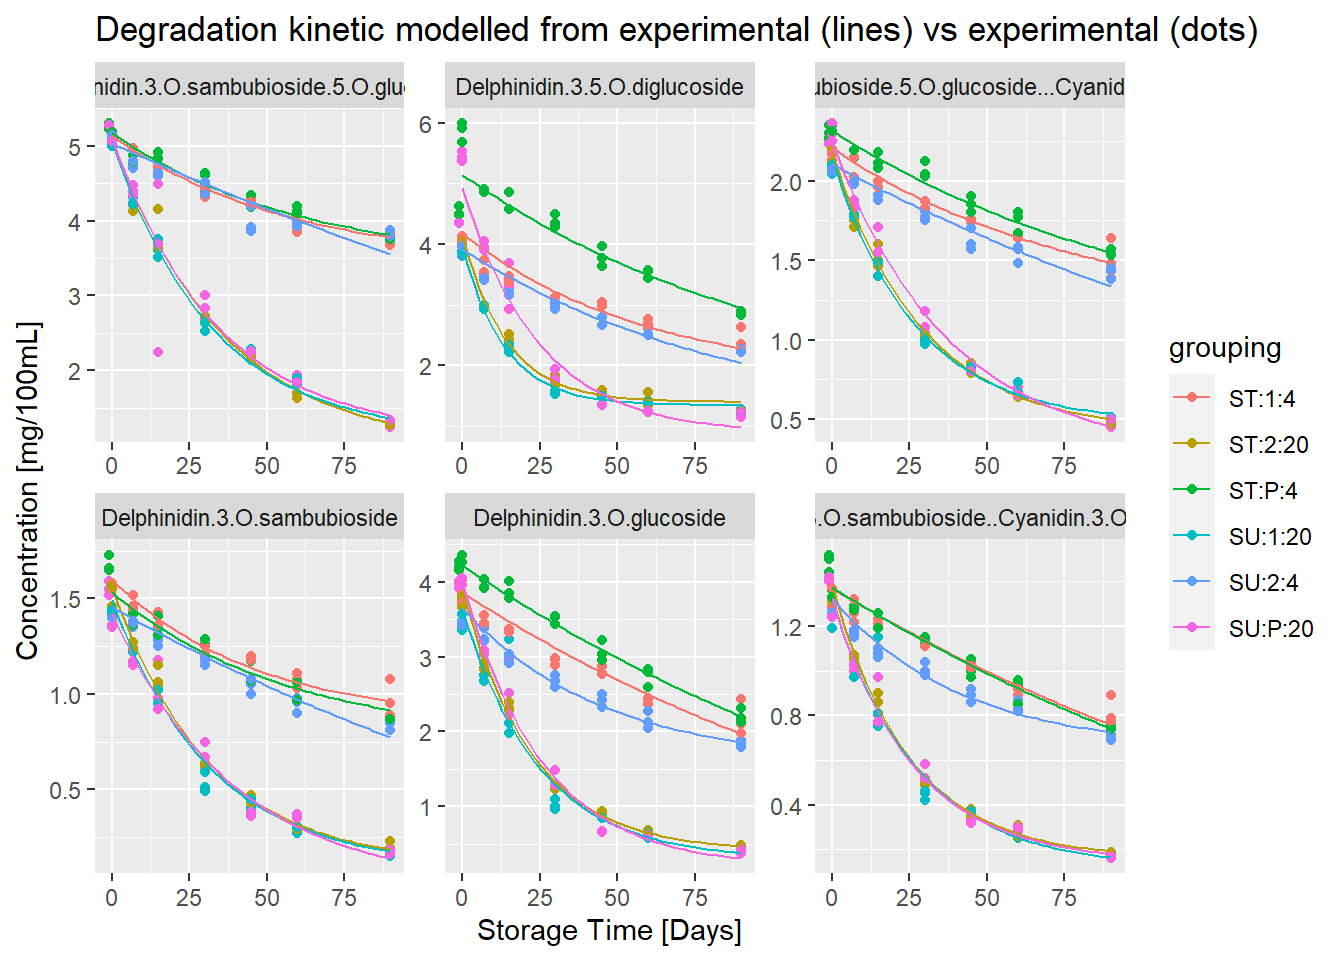
\includegraphics{firstModel_Jesus_files/figure-latex/figure of predictions-1.pdf}

\begin{Shaded}
\begin{Highlighting}[]
\FunctionTok{ggsave}\NormalTok{(}\AttributeTok{filename=}\StringTok{"Figure1.pdf"}\NormalTok{)}
\end{Highlighting}
\end{Shaded}

\begin{verbatim}
## Saving 6.5 x 4.5 in image
\end{verbatim}

Podemos concluir que este cuarto modelo ajusta bastante bien la
degradación del compuesto respecto a los datos experimentales salvo
algún punto marginal, y que puede emplearse para realizar predicciones
bastante ajustadas en el caso de los antocianos.

Por tanto, repetimos el proceso de ajuste y modelado con las condiciones
de las cuales carecemos de datos experimentales, para posteriormente
compararlas.

\begin{verbatim}
##               Model df       AIC       BIC   logLik   Test  L.Ratio p-value
## ant.fm0_pred2     1 25   71.2563  190.2956 -10.6282                        
## ant.fm3_pred2     2 79 -633.2143 -257.0501 395.6072 1 vs 2 812.4706  <.0001
\end{verbatim}

\begin{verbatim}
## [1] 0.9887058 0.9875993
\end{verbatim}

\includegraphics{firstModel_Jesus_files/figure-latex/modelo sin datos-1.pdf}
\includegraphics{firstModel_Jesus_files/figure-latex/modelo sin datos-2.pdf}
\includegraphics{firstModel_Jesus_files/figure-latex/modelo sin datos-3.pdf}
\includegraphics{firstModel_Jesus_files/figure-latex/modelo sin datos-4.pdf}
\includegraphics{firstModel_Jesus_files/figure-latex/modelo sin datos-5.pdf}
\includegraphics{firstModel_Jesus_files/figure-latex/modelo sin datos-6.pdf}

\begin{verbatim}
## The table was written to the file 'anthocyanins_pred2.html'.
\end{verbatim}

\includegraphics{firstModel_Jesus_files/figure-latex/modelo sin datos 2-1.pdf}

\begin{verbatim}
## Saving 6.5 x 4.5 in image
\end{verbatim}

Podemos concluir que el ajuste y las pruebas nos dicen que el modelo es
válido para las condiciones dadas, como en el caso anterior.

Ahora procedemos a comparar el ajuste de los datos experimentales a las
predicciones que realiza el mismo modelo sobre las condiciones de las
que no disponemos de datos experimentales.

\begin{Shaded}
\begin{Highlighting}[]
\CommentTok{\# ST:1}

\FunctionTok{ggplot}\NormalTok{(}\AttributeTok{data =}\NormalTok{ ant.pred2 }\SpecialCharTok{\%\textgreater{}\%} \FunctionTok{filter}\NormalTok{(grouping }\SpecialCharTok{==} \StringTok{"ST:1:20"}\NormalTok{), }\FunctionTok{aes}\NormalTok{(}\AttributeTok{x=}\NormalTok{tiempo, }\AttributeTok{y =}\NormalTok{ concentration, }\AttributeTok{col =}\NormalTok{ Temp))}\SpecialCharTok{+}
       \FunctionTok{facet\_wrap}\NormalTok{(compound}\SpecialCharTok{\textasciitilde{}}\NormalTok{.,}\AttributeTok{scales=}\StringTok{"free"}\NormalTok{)}\SpecialCharTok{+}
       \FunctionTok{geom\_point}\NormalTok{()}\SpecialCharTok{+}\FunctionTok{geom\_line}\NormalTok{(}\AttributeTok{data=}\NormalTok{ant.pred }\SpecialCharTok{\%\textgreater{}\%} \FunctionTok{filter}\NormalTok{(grouping }\SpecialCharTok{==} \StringTok{"ST:1:4"}\NormalTok{), }\FunctionTok{aes}\NormalTok{(}\AttributeTok{x=}\NormalTok{tiempo, }\AttributeTok{y=}\NormalTok{concentration, }\AttributeTok{col =}\NormalTok{ Temp))}\SpecialCharTok{+}
  \FunctionTok{ggtitle}\NormalTok{(}\StringTok{"ST:P 20º modelled (points) | 4º experimental (line)"}\NormalTok{) }\SpecialCharTok{+} \FunctionTok{xlab}\NormalTok{(}\StringTok{"Storage Time [Days]"}\NormalTok{)}\SpecialCharTok{+}\FunctionTok{ylab}\NormalTok{(}\StringTok{"Concentration [mg/100mL]"}\NormalTok{)}
\end{Highlighting}
\end{Shaded}

\begin{center}\includegraphics{firstModel_Jesus_files/figure-latex/comparación predicciones-1} \end{center}

\begin{Shaded}
\begin{Highlighting}[]
\CommentTok{\# ST:2}
\FunctionTok{ggplot}\NormalTok{(}\AttributeTok{data =}\NormalTok{ ant.pred2 }\SpecialCharTok{\%\textgreater{}\%} \FunctionTok{filter}\NormalTok{(grouping }\SpecialCharTok{==} \StringTok{"ST:2:4"}\NormalTok{), }\FunctionTok{aes}\NormalTok{(}\AttributeTok{x=}\NormalTok{tiempo, }\AttributeTok{y =}\NormalTok{ concentration, }\AttributeTok{col =}\NormalTok{ Temp))}\SpecialCharTok{+}
  \FunctionTok{facet\_wrap}\NormalTok{(compound}\SpecialCharTok{\textasciitilde{}}\NormalTok{.,}\AttributeTok{scales=}\StringTok{"free"}\NormalTok{)}\SpecialCharTok{+}
  \FunctionTok{geom\_point}\NormalTok{()}\SpecialCharTok{+}\FunctionTok{geom\_line}\NormalTok{(}\AttributeTok{data=}\NormalTok{ant.pred }\SpecialCharTok{\%\textgreater{}\%} \FunctionTok{filter}\NormalTok{(grouping }\SpecialCharTok{==} \StringTok{"ST:2:20"}\NormalTok{), }\FunctionTok{aes}\NormalTok{(}\AttributeTok{x=}\NormalTok{tiempo, }\AttributeTok{y=}\NormalTok{concentration, }\AttributeTok{col =}\NormalTok{ Temp))}\SpecialCharTok{+}
  \FunctionTok{ggtitle}\NormalTok{(}\StringTok{"SU:1 20º experimental (lineal) | 4º modelled (points)"}\NormalTok{)}\SpecialCharTok{+} \FunctionTok{xlab}\NormalTok{(}\StringTok{"Storage Time [Days]"}\NormalTok{)}\SpecialCharTok{+}\FunctionTok{ylab}\NormalTok{(}\StringTok{"Concentration [mg/100mL]"}\NormalTok{)}
\end{Highlighting}
\end{Shaded}

\begin{center}\includegraphics{firstModel_Jesus_files/figure-latex/comparación predicciones-2} \end{center}

\begin{Shaded}
\begin{Highlighting}[]
\CommentTok{\# ST:P}
\FunctionTok{ggplot}\NormalTok{(}\AttributeTok{data =}\NormalTok{ ant.pred2 }\SpecialCharTok{\%\textgreater{}\%} \FunctionTok{filter}\NormalTok{(grouping }\SpecialCharTok{==} \StringTok{"ST:P:20"}\NormalTok{), }\FunctionTok{aes}\NormalTok{(}\AttributeTok{x=}\NormalTok{tiempo, }\AttributeTok{y =}\NormalTok{ concentration, }\AttributeTok{col =}\NormalTok{ Temp))}\SpecialCharTok{+}
  \FunctionTok{facet\_wrap}\NormalTok{(compound}\SpecialCharTok{\textasciitilde{}}\NormalTok{.,}\AttributeTok{scales=}\StringTok{"free"}\NormalTok{)}\SpecialCharTok{+}
  \FunctionTok{geom\_point}\NormalTok{()}\SpecialCharTok{+}\FunctionTok{geom\_line}\NormalTok{(}\AttributeTok{data=}\NormalTok{ant.pred }\SpecialCharTok{\%\textgreater{}\%} \FunctionTok{filter}\NormalTok{(grouping }\SpecialCharTok{==} \StringTok{"ST:P:4"}\NormalTok{), }\FunctionTok{aes}\NormalTok{(}\AttributeTok{x=}\NormalTok{tiempo, }\AttributeTok{y=}\NormalTok{concentration, }\AttributeTok{col =}\NormalTok{ Temp))}\SpecialCharTok{+}
  \FunctionTok{ggtitle}\NormalTok{(}\StringTok{"ST:P 20º modelled (points) | 4º experimental (line)"}\NormalTok{)}\SpecialCharTok{+} \FunctionTok{xlab}\NormalTok{(}\StringTok{"Storage Time [Days]"}\NormalTok{)}\SpecialCharTok{+}\FunctionTok{ylab}\NormalTok{(}\StringTok{"Concentration [mg/100mL]"}\NormalTok{)}
\end{Highlighting}
\end{Shaded}

\begin{center}\includegraphics{firstModel_Jesus_files/figure-latex/comparación predicciones-3} \end{center}

\begin{Shaded}
\begin{Highlighting}[]
\CommentTok{\# SU:1}

\FunctionTok{ggplot}\NormalTok{(}\AttributeTok{data =}\NormalTok{ ant.pred2 }\SpecialCharTok{\%\textgreater{}\%} \FunctionTok{filter}\NormalTok{(grouping }\SpecialCharTok{==} \StringTok{"SU:1:4"}\NormalTok{), }\FunctionTok{aes}\NormalTok{(}\AttributeTok{x=}\NormalTok{tiempo, }\AttributeTok{y =}\NormalTok{ concentration, }\AttributeTok{col =}\NormalTok{ Temp))}\SpecialCharTok{+}
  \FunctionTok{facet\_wrap}\NormalTok{(compound}\SpecialCharTok{\textasciitilde{}}\NormalTok{.,}\AttributeTok{scales=}\StringTok{"free"}\NormalTok{)}\SpecialCharTok{+}
  \FunctionTok{geom\_point}\NormalTok{()}\SpecialCharTok{+}\FunctionTok{geom\_line}\NormalTok{(}\AttributeTok{data=}\NormalTok{ant.pred }\SpecialCharTok{\%\textgreater{}\%} \FunctionTok{filter}\NormalTok{(grouping }\SpecialCharTok{==} \StringTok{"SU:1:20"}\NormalTok{), }\FunctionTok{aes}\NormalTok{(}\AttributeTok{x=}\NormalTok{tiempo, }\AttributeTok{y=}\NormalTok{concentration, }\AttributeTok{col =}\NormalTok{ Temp)) }\SpecialCharTok{+}
  \FunctionTok{ggtitle}\NormalTok{(}\StringTok{"SU:1 20º experimental (line) | 4º modelled (points)"}\NormalTok{)}\SpecialCharTok{+} \FunctionTok{xlab}\NormalTok{(}\StringTok{"Storage Time [Days]"}\NormalTok{)}\SpecialCharTok{+}\FunctionTok{ylab}\NormalTok{(}\StringTok{"Concentration [mg/100mL]"}\NormalTok{)}
\end{Highlighting}
\end{Shaded}

\begin{center}\includegraphics{firstModel_Jesus_files/figure-latex/comparación predicciones-4} \end{center}

\begin{Shaded}
\begin{Highlighting}[]
\CommentTok{\# SU:2}

\FunctionTok{ggplot}\NormalTok{(}\AttributeTok{data =}\NormalTok{ ant.pred2 }\SpecialCharTok{\%\textgreater{}\%} \FunctionTok{filter}\NormalTok{(grouping }\SpecialCharTok{==} \StringTok{"SU:2:20"}\NormalTok{), }\FunctionTok{aes}\NormalTok{(}\AttributeTok{x=}\NormalTok{tiempo, }\AttributeTok{y =}\NormalTok{ concentration, }\AttributeTok{col =}\NormalTok{ Temp))}\SpecialCharTok{+}
  \FunctionTok{facet\_wrap}\NormalTok{(compound}\SpecialCharTok{\textasciitilde{}}\NormalTok{.,}\AttributeTok{scales=}\StringTok{"free"}\NormalTok{)}\SpecialCharTok{+}
  \FunctionTok{geom\_point}\NormalTok{()}\SpecialCharTok{+}\FunctionTok{geom\_line}\NormalTok{(}\AttributeTok{data=}\NormalTok{ant.pred }\SpecialCharTok{\%\textgreater{}\%} \FunctionTok{filter}\NormalTok{(grouping }\SpecialCharTok{==} \StringTok{"SU:2:4"}\NormalTok{), }\FunctionTok{aes}\NormalTok{(}\AttributeTok{x=}\NormalTok{tiempo, }\AttributeTok{y=}\NormalTok{concentration, }\AttributeTok{col =}\NormalTok{ Temp)) }\SpecialCharTok{+}
  \FunctionTok{ggtitle}\NormalTok{(}\StringTok{"SU:2 20º modelled (points) | 4º experimental (lines)"}\NormalTok{)}\SpecialCharTok{+} \FunctionTok{xlab}\NormalTok{(}\StringTok{"Storage Time [Days]"}\NormalTok{)}\SpecialCharTok{+}\FunctionTok{ylab}\NormalTok{(}\StringTok{"Concentration [mg/100mL]"}\NormalTok{)}
\end{Highlighting}
\end{Shaded}

\begin{center}\includegraphics{firstModel_Jesus_files/figure-latex/comparación predicciones-5} \end{center}

\begin{Shaded}
\begin{Highlighting}[]
\CommentTok{\# SU:P}

\FunctionTok{ggplot}\NormalTok{(}\AttributeTok{data =}\NormalTok{ ant.pred2 }\SpecialCharTok{\%\textgreater{}\%} \FunctionTok{filter}\NormalTok{(grouping }\SpecialCharTok{==} \StringTok{"SU:P:4"}\NormalTok{), }\FunctionTok{aes}\NormalTok{(}\AttributeTok{x=}\NormalTok{tiempo, }\AttributeTok{y =}\NormalTok{ concentration, }\AttributeTok{col =}\NormalTok{ Temp))}\SpecialCharTok{+}
  \FunctionTok{facet\_wrap}\NormalTok{(compound}\SpecialCharTok{\textasciitilde{}}\NormalTok{.,}\AttributeTok{scales=}\StringTok{"free"}\NormalTok{)}\SpecialCharTok{+}
  \FunctionTok{geom\_point}\NormalTok{()}\SpecialCharTok{+}\FunctionTok{geom\_line}\NormalTok{(}\AttributeTok{data=}\NormalTok{ant.pred }\SpecialCharTok{\%\textgreater{}\%} \FunctionTok{filter}\NormalTok{(grouping }\SpecialCharTok{==} \StringTok{"SU:P:20"}\NormalTok{), }\FunctionTok{aes}\NormalTok{(}\AttributeTok{x=}\NormalTok{tiempo, }\AttributeTok{y=}\NormalTok{concentration, }\AttributeTok{col =}\NormalTok{ Temp)) }\SpecialCharTok{+}
  \FunctionTok{ggtitle}\NormalTok{(}\StringTok{"SU:P 20º experimental (line) | 4º modelled (points)"}\NormalTok{)}\SpecialCharTok{+} \FunctionTok{xlab}\NormalTok{(}\StringTok{"Storage Time [Days]"}\NormalTok{)}\SpecialCharTok{+}\FunctionTok{ylab}\NormalTok{(}\StringTok{"Concentration [mg/100mL]"}\NormalTok{)}
\end{Highlighting}
\end{Shaded}

\begin{center}\includegraphics{firstModel_Jesus_files/figure-latex/comparación predicciones-6} \end{center}

\end{document}
